\documentclass[12pt,final]{article}
% \usepackage{pdflscape}
\usepackage{pdfpages}

\usepackage{epstopdf}
\epstopdfDeclareGraphicsRule{.tiff}{png}{.png}{convert -density 180 #1 \OutputFile}
\AppendGraphicsExtensions{.tiff}


\author{Nico Albers}
\title{Abgabe 0 Autonomes Fahren}
\begin{document}
\maketitle

\section{Aufgabe 0}
Die maximale Geschwindigkeit, bis zu der die Simulation nicht ins Schleudern gerät, liegt bei $7\frac{m}{s}$.

Sobald die Geschwindigkeit höher liegt, passiert in einer der Kurven folgendes:
Innerhalb der im letzten Schritt gefundenen Fahrbahnbegrenzungen liegt keine
Fahrbahn mehr und durch die fehlenden weißen Pixel innerhalb dieser Fahrbahnbegrenzungen
schlägt die Methode zur Winkelbestimmung fehl.

Vergleiche im Folgenden eine durchgeführte Messung.
Die Mittellinie ist im Hintergrund etwas breiter in grau zu sehen -- wenn der
Wagen also an den Rand dieser breiten Mittellinie kommt ist er über die eigentliche
schon deutlich hinaus.

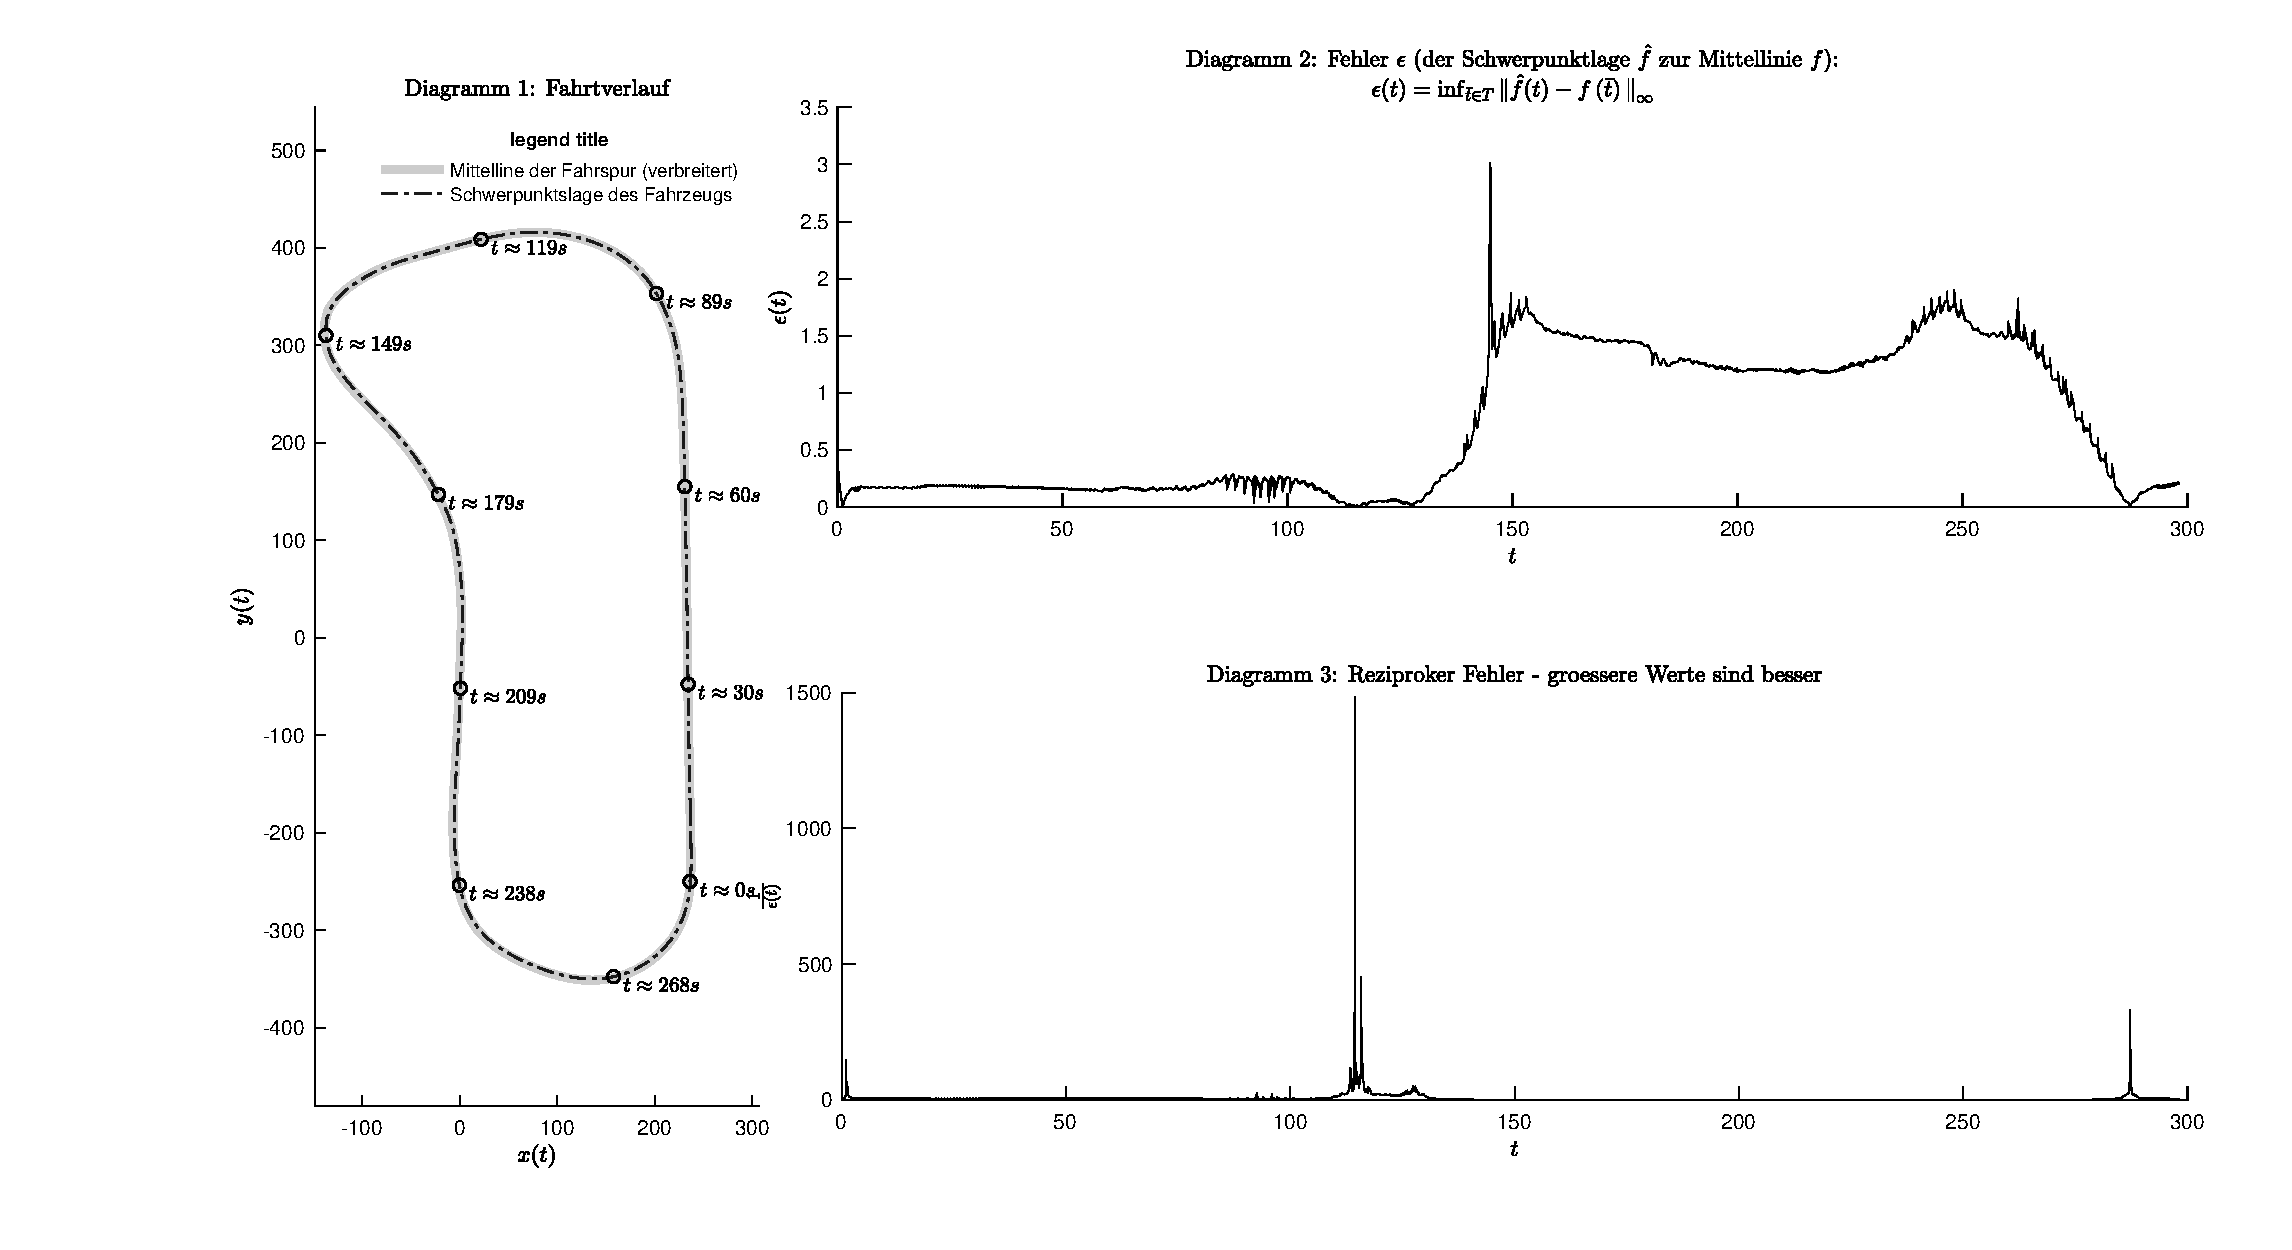
\includepdf[noautoscale=false,fitpaper=true,landscape]{ex01_measured_track.pdf}
\includepdf[noautoscale=false,fitpaper=true,landscape]{ex01_screenshot.tiff}

\end{document}
